\documentclass[12pt,a4paper]{article}

\usepackage{amsfonts,amssymb,amsmath,amsthm}
\usepackage{stmaryrd} %for special brackets
\usepackage{lipsum}
\usepackage{graphicx}
\graphicspath{img}
\usepackage[hidelinks]{hyperref}
\usepackage{array}
\usepackage{bm} %for bold in math equations
\usepackage{float} %to force the position of some figures
\usepackage{biblatex}
\usepackage{geometry}
\usepackage{todonotes}


\addbibresource{_report.bib}
\geometry{left=2.54cm,right=2.54cm}


\title{Internship Report}
\author{Lucas SALAND}
\date{\today}

\begin{document}
\maketitle
\newpage
\tableofcontents
\newpage

\section*{Introduction}
This M1 internship was carried out at CRIStAL in the SIGMA team under the supervision of Patrick Bas. The internship lasted for three months during which we worked on a challenge from the AID on the detection of images generated by AI.

\subsection*{Work environment : CRIStAL and SIGMA}
CRIStAL is a laboratory which research focus on computer science, signal and automatic control. It is under the supervision of the University of Lille, CNRS and Centrale Lille. The laboratory is divided in 34 research teams grouped in 9 Thematic Groups. SIGMA team is part of DatInG : Data Intelligence Group. SIGMA is a team of 15 permanent staff which focuses on machine learning, statistics and signal processing. Some of the research topics are Monte-Carlo methods, signal processing with tensorial approaches and information security.

\subsection*{The challenge from AID}
The Agence de l'innovation et de défense (AID) launched a challenge on détecting modified or generated images. This challenge aimed at detecting three types of images :
\begin{itemize}
    \item fully AI-generated images;
    \item images partially modified by AI;
    \item images partially modified with more usual image processing tools such as photoshop.
\end{itemize}
This challenge was divided in two tasks : A and B. Task A focused on images fully generated by AI. AID would provide 10000 images. The goal was to identify which images were real and which one were generated. On top of this, we could provide which generator was used to generate images. Task A could be treated as binary classification problem with the two classes being real and generated images. It could also be treated as a multi-class classification problem where the classes would be the real images and all the generator used. The main difficulty was that the generators used were kept secret until the last day of the challenge.\\
Task B focused on the detection of partially modified images. The objectives were :
\begin{itemize}
    \item detecting real images and modified images;
    \item identifying the tool used for modification;
    \item localisation of modification on images.
\end{itemize}

I worked on the challenge in a team with 3 other interns and 5 permanent staff from SIGMA. During the internship, I worked on task A.

\subsection*{AI image generation}
We should now go over an overview of image generation with AI. In recent years, the quality of images generated with AI models skyrocketed. These models appear as promising new tools for art generation and data augmentation for machine learning. In 2014, Generative Adversarial Networks were introduced by Ian J. Goodfellow and his colleagues in \autocite*{goodfellowGenerativeAdversarialNetworks2014}. A GAN is composed of two main components : a generator and a discriminator. The generator take random vector as input and tries to generate images that are indistinguishable from real images. It tries to fool the discriminator. On the other hand, the discriminator's goal is to differentiate between real data from the training set and fake data produced by the generator.
\begin{figure}[H]
    \centering
    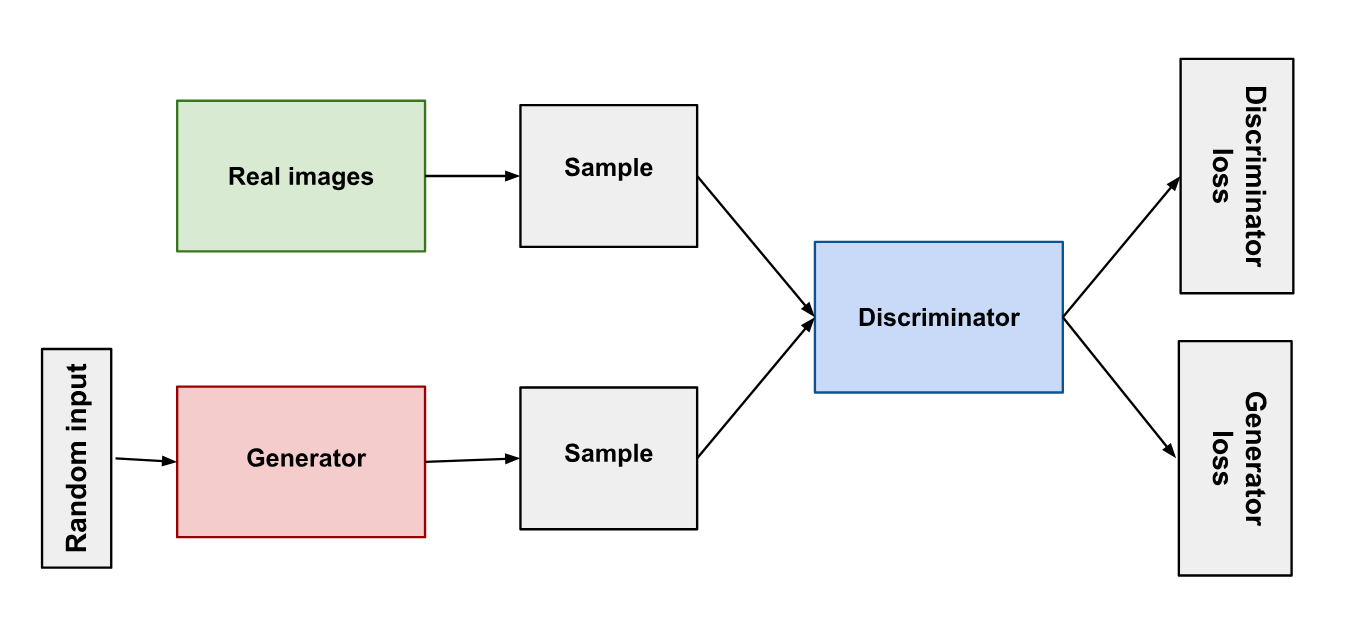
\includegraphics[width=\textwidth]{img/GAN.png}
    \caption{GAN architecture}
\end{figure}

Diffusion models use a different approach to generate images.
\todo[inline]{More on diffusion model}

\section{AI-generated images detection}
As improvements happen at an impressive rate in the field of generative models, concerns about security issues rose as well. These tools could be used to manipulate information and combined with social media they would be weapon of massive disinformation. As generative model keep improving, we need to develop new tools to detect generated images. But what should we look for in generated images in order to differentiate them from real images? To develop an efficient detector, we decided to explore a semantic approach. Let's first give a definition of semantic. For an image, the semantic refers to the content of the image. The objects and things that are perceived by the humans. Images generated by AI tend to have a poor semantic content in comparison to real images. But how should we process images to extract their semantic content? That's where image encoders come into play. More specifically CLIP's image encoder.

\subsection{CLIP}
\autocite*{cozzolinoRaisingBarAIgenerated2024}
\subsection{Impact of JPEG compression}
\subsection{Adding diversity to the data}
\subsection{Bigger datasets and neural network}
\subsection{Pair training}
\subsection{Filling the holes with fine tuning}

\section{Additional explorations}
\subsection{Color features}

\subsection{DINO as an alternative to CLIP}
\autocite*{oquabDINOv2LearningRobust2024}

\subsection{Tip-Adapter}
\autocite*{khanCLIPpingDeceptionAdapting2024}
\autocite*{zhangTipAdapterTrainingfreeAdaption2022}
\subsection{Understanding CLIP features}
AID real img are bad crops with poor semantic content so why does CLIP detector performed well ?
Adversarial attack.

\section*{Conclusion}

\newpage
\printbibliography

\end{document}